%% fancy header & foot
\pagestyle{fancy}
\lhead{[ELEC-H-2001] Électricité  \ifthenelse{\boolean{corrige}}{~-- corrigé}{}}
\rhead{v1.0.2\\ page \thepage}
\cfoot{}
%%

\pdfinfo{
/Author (Raoul Sommeillier, ULB -- BEAMS)
/Title (ELEC-H-2001, Théorie des champs Électrostatique : champ et potentiel dans le vide)
/ModDate (D:\pdfdate)
}

\hypersetup{
pdftitle={[ELEC-H-2001] Électricité Théorie des champs\\Électrostatique : champ et potentiel dans le vide},
pdfauthor={Raoul Sommeillier, ©2018 ULB - BEAMS  },
%pdfsubject={Théorie des champs\\Électrostatique : champ et potentiel dans le vide}
}

%\date{\vspace{-1cm}\mydate\today}
%\title{\vspace{-2cm} Labo \no 6\\ Électronique appliquée [ELEC-H-301]\\Réalisation d'un ampli à transistor\ifthenelse{\boolean{corrige}}{~\\Corrigé}{}}

%\author{\vspace{-1cm}}%\textsc{Yannick Allard}}

\setlength{\parskip}{0.5cm plus4mm minus3mm} %espacement entre §
\setlength{\parindent}{0pt}


\begin{document}

\tptitle{}{Électrostatique : champ et potentiel dans le vide}

\section{Pré-requis et objectif de la séance}
Avant cette séance, il est préférable d'avoir lu attentivement cet énoncé et revu les chapitres du cours couvrant la théorie vue dans les 4 premières séances d'exercices en Théorie des Circuits.

Les compétences devant être développées par l'étudiant à la fin de cette séance sont en particulier:
\begin{itemize}
	\item Analyser un circuit quelconque et combiner vos connaissances afin de sélectionner la procédure adéquate pour le résoudre
	\item Driller vos connaissances et savoir-faire sur les matières vues précédemment aux séances d'exercices 1 à 4, à savoir: les impédances, les circuits passifs ou réactifs à une ou plusieurs source(s) continue(s) ou alternative(s) en régime transitoire ou établi, les lois de Kirchhoff, les théorèmes de Thévenin et de superposition, l'adaptation d'impédance, le formalisme des phaseurs, etc.  
\end{itemize}

Cet énoncé étant long, vous aurez l'occasion de travailler dessus avec vos assistants à la fin des séances de laboratoire.
\vspace{5pt}

\newpage

\section{Exercices}
\subsection{Soient quatre charges $q_{1}$, $q_{2}$, $q_{3}$, $q_{4}$, disposées de manière à former un carré de côté de longueur $a$.}
\begin{figure}[h!]
    \centering
    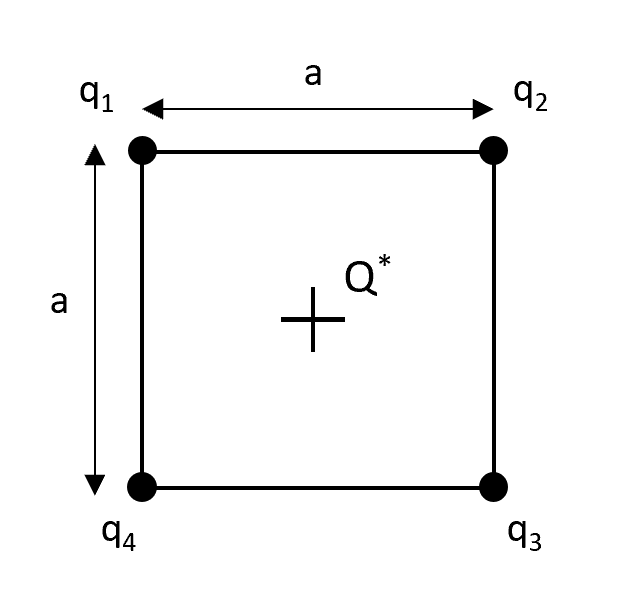
\includegraphics[width = 8cm]{TP5/Tp5_Q1.PNG}
    \caption{Répartition des quatre charges}
    \label{fig:Q1Enonce}
\end{figure}
\Question{ Si les charges ont une même valeur (par exemple: $q_1 = q_2 = q_3 = q_4 = +q$), calculez :
    \begin{itemize}
        \item Le potentiel électrique $\mathbf{V}$ généré par ces dernières au centre du carré.
        \item La force résultante $\mathcal{F}_{res}$ qu'exercent ces quatre charges sur une charge témoin $\mathbf{Q^*}$ placée au centre du carré.
        \item Le travail $\mathcal{W}$ nécessaire pour amener la charge témoin $\mathbf{Q^*}$ d'un point infiniment éloigné jusqu'au centre du carré.
        \item Que devient cette force si une des charges positionnées aux sommets du carré venait à être retirée?
    \end{itemize}
    }
    {}

\Question{Si les charges sont alternées en signe (par exemple : $q_1 = q_3 = +q$ et $q_2 = q_4 = -q$), calculez : 
    \begin{itemize}
        \item Le potentiel électrique $\mathbf{V}$ généré par ces dernières au centre du carré.
        \item La force résultante $\mathcal{F}_{res}$ qu'exercent ces quatre charges sur une charge témoin $\mathbf{Q^*}$ placée au centre du carré.
        \item Le travail $\mathcal{W}$ nécessaire pour amener la charge témoin $\mathbf{Q^*}$ d'un point infiniment éloigné jusqu'au centre du carré.
        \item Que devient cette force si une des charges positionnées aux sommets du carré venait à être retirée?
    \end{itemize}
    }
    {}

\subsection{On considère deux charges Q et -Q distantes d'une longueur s. Les charges sont alignées suivant l'axe x et symétriquement par rapport à l'origine du système d'axes, tel que représenté sur le schéma ci-dessous:}
\begin{figure}[h!]
    \centering
    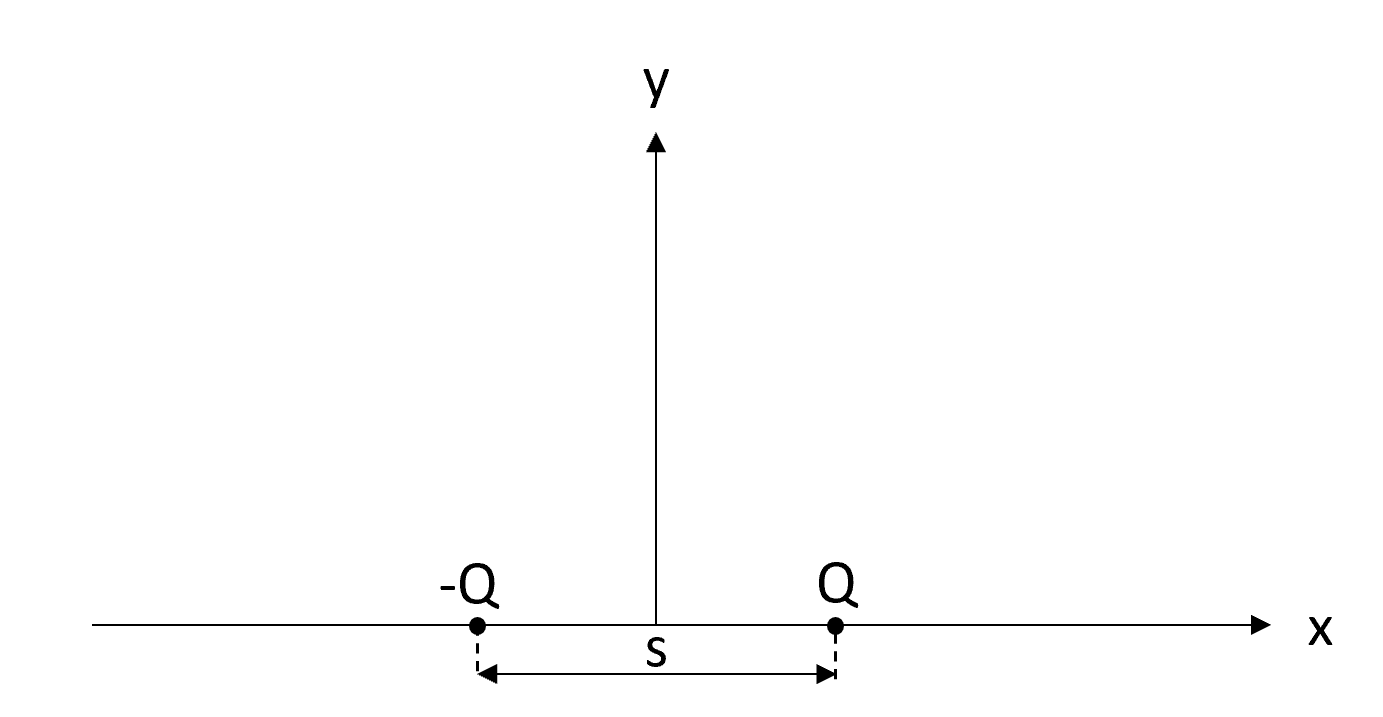
\includegraphics[width = 8cm]{TP5/Tp5_Q2.PNG}
    \caption{Disposition des charges}
    \label{fig:Q2Ennonce}
\end{figure}
\Question{
\begin{itemize}
    \item Déterminez l'expression analytique du champ électrique $\mathbf{E}$ selon l'axe $x$ puis selon l'axe $y$
    \item Simplifiez ces expressions en considérant que la distance aux charges est beaucoup plus grande que $s$ (approximation dipolaire).
    \item Dessinez l'allure des lignes de champ dans le plan xy.
\end{itemize} 
}
{}

\subsection{Considérons une sphère de rayon a portant une charge \textit{totale} Q.}
\Question{Déterminez analytiquement la répartition du potentiel électrique $\mathbf{V}$ et du champ électrique associé $\Vec{E}$ pour tous rayon partant du centre de la sphère jusqu'à l'infini pour les distributions de charge suivantes:
\begin{itemize}
    \item Si la charge $\mathbf{Q}$ est répartie uniformément en volume dans la sphère.
    \item Si la charge $\mathbf{Q}$ est répartie uniformément en surface de la sphère.
    \item Si la charge $\mathbf{Q}$ est répartie dans le volume de la sphère suivant une loi proportionnelle à $R^2$.
\end{itemize}
}
{}
\subsection{Soit un anneau circulaire \textit{filiforme} de diamètre \textit{d} portant une densité de charge linéaire et uniforme $\rho_L$ en $C/m$.}
\Question{Déterminez le potentiel électrique $\mathbf{V}$ et le champ électrique $\Vec{E}$ au centre de cet anneau.}
{}


%QUESTION 9
\Question{
\textit{Résoudre ce circuit où $E_S=10V$. On ferme le premier interrupteur au temps $t=T_1$, puis le second au temps $t=T_2$.\\
On supposera le temps $T_2-T_1$ bien plus grands que les constantes de temps de ce circuit.}
\begin{center}
\begin{circuitikz} \draw
(0,0)   node [ground] {}
		to [american voltage source, v=$E$, invert] 		(0,3)
		to [closing switch, l=$T_1$]				(2,3)
		to [R, l=$R$]								(5,3)
		to [C, l=$C$]								(5,0)
		--(0,0)
(5,3)	to[closing switch, l=$T_2$]					(7,3)
		to [R, l=$R_2$]								(7,0)--(5,0)
;
\end{circuitikz}
\end{center}
}
{
Avant $T_2$, c'est le même circuit que la question 3 de cet exercice: $v_C(t)=E_S(1-e^{\frac{-t}{RC}})$.\\
Après $T_2$, c'est le même exercice que le 2.6 du TP2.
}

%QUESTION 2.2.
\subsection{Question de l'Examen de Janvier 2013}
Soit le circuit suivant
\begin{center}
\begin{circuitikz} \draw
(0,0)   node [ground] {}
		to	 [american voltage source, v=$E$, invert]	(0,2)
		to	 [R, l=$r$]							(0,4)--(2,4)
(2,0)	to	 [american voltage source, v=$2E$, invert]	(2,2)
		to	 [R, l=$r$]							(2,4)--(4,4)
(4,0)	to	 [american voltage source, v=$3E$, invert]	(4,2)
		to	 [R, l=$r$]							(4,4)--(6,4)
(6,0)		to	 [american voltage source, v=$4E$, invert]	(6,2)
		to	 [R, l=$r$]							(6,4)
		to	 [closing switch]					(8,4)
		to   [R, l=$R$]							(8,2)
		to   [C, l=$C$]							(8,0)--(0,0)	
;
\end{circuitikz}
\end{center}

Où $E=20V$, $r=4\Omega$, $R=1\Omega$ et $0,1F$.\\
Avant $t=0$, l'interrupteur est ouvert. On ferme l'interrupteur à l'instant $t=0$. La charge initiale de la capacité est nulle.\\

Après une prise de mesure, on a relevé les deux courbes suivantes où l'axe des abscisses est le temps $[s]$ (une graduation vaut $0,2s$) et l'axe des ordonnées est le courant $[A]$ ou la tension $[V]$.
\begin{center}
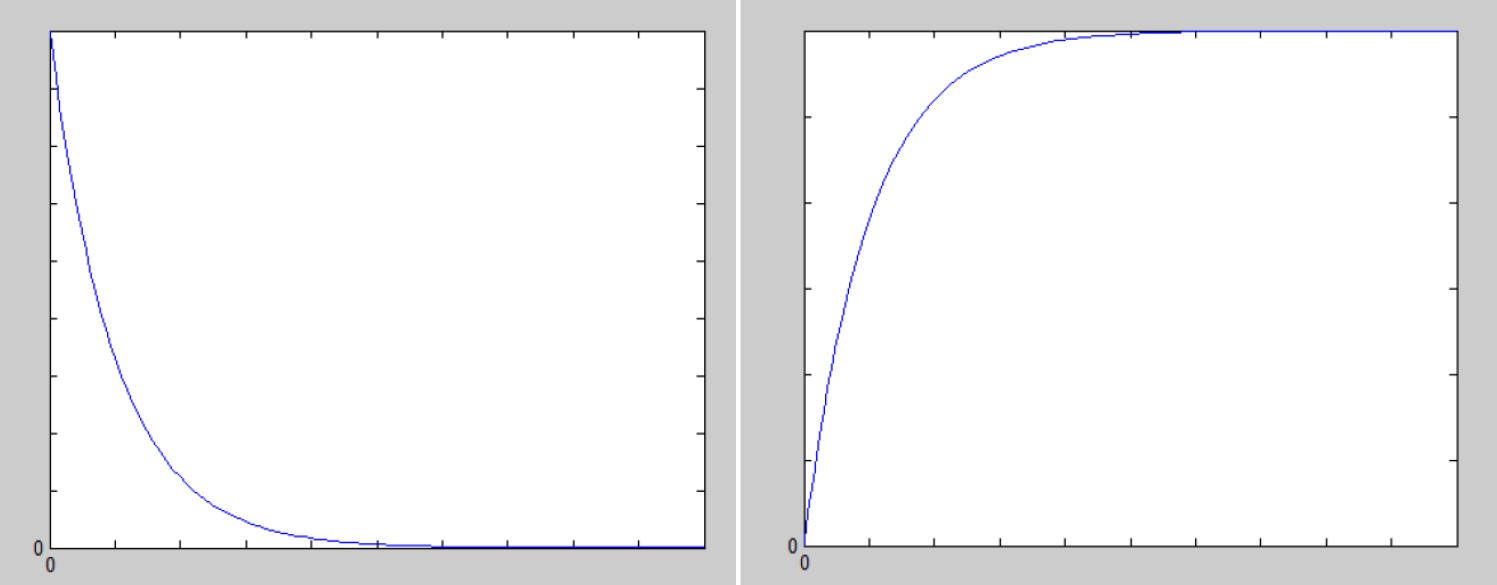
\includegraphics[scale=0.4]{TP5/RC.PNG}
\end{center}

%QUESTION 1.1.
\Question
{
%question
\textit{Identifiez l'élément du schéma (source(s), capacité, resistance(s)) auquel se rapportent ces deux graphes.\\
Identifiez la grandeur (tension(s) ou courant(s)) présente sur l'ordonnée pour chaque courbe.}
}
{
\textbf{Elément:} La capacité\\

\textbf{A droite:}\\
Il s'agit de la tension aux bornes du condensateur $v_C(t)$.\\

Vérification numérique après résolution de la Question 1.4.:\\
$v_C(t)=\frac{5E}{2}(1-\exp{(-\frac{t}{C(R+r/4)})})=50(1-\exp{(-\frac{t}{0,2})}) [V]$ avec une tension initiale $v_C(0-)=v_C(0+)=0V$ et une tension de régime $v_C(\infty)=50V$\\


\textbf{A gauche:}\\
Il s'agit de l'intensité de courant $i(t)$ traversant le condensateur.\\

Vérification numérique après résolution de la Question 1.4.:\\
$i(t)=\frac{10E}{4R+r}exp{(-\frac{t}{C(R+r/4)})}=25 exp{(-\frac{t}{0,2})} [A]$ avec $i(0-)=0A$, $i(0+)=25A$ et $i(\infty)=0A$.
}


%QUESTION 1.2.
\Question
{
%question
\textit{Sur base de ce graphique, déterminer la valeur de la constante de temps $\tau$ du circuit.}
}
{
La constante de temps $\tau$ est par définition le temps nécessaire à la tension aux bornes du condensateur pour atteindre $63\%$ de sa valeur de régime:
$$v_C(\tau)=v_C(\infty)(1-\exp{(-1}))\cong 0,63v_C(\infty)$$

Graphiquement, il suffit de tracer une ligne horizontale passant par $0,63\times 50=31,5V$.\\ L'intersection avec le graphique de $v_C(t)$ donne $\tau=0,2s$.\\

Il était également possible d'utiliser la méthode graphique de la tangente à l'origine (moins précis).

Vérification numérique après résolution:
$$\tau=C(R+\frac{r}{4})=0,1.(1+\frac{4}{4})=0,2s$$
}

%QUESTION 1.3.
\Question
{
%question
\textit{Déterminez les paramètres $R_{th}$ et $V_{th}$ de l'équivalent de Thévenin du circuit vu aux bornes du condensateur.}
}
{
\fbox{$R_{th}$}\\
Pour trouver la résistance équivalente de Thévenin, il faut court-circuiter les sources du circuit. (1 point)

\begin{center}
\begin{circuitikz}[scale=0.6] \draw
(0,0)   node [ground] {}
		to	 [short]	(0,2)
		to	 [R, l=$r$]							(0,4)--(2,4)
(2,0)	to	 [short]	(2,2)
		to	 [R, l=$r$]							(2,4)--(4,4)
(4,0)	to	 [short]	(4,2)
		to	 [R, l=$r$]							(4,4)--(6,4)
(6,0)	to	 [short]	(6,2)
		to	 [R, l=$r$]							(6,4)
		to	 [short]					(8,4)
		to   [R, l=$R$]							(8,2)
		to   [open, l=$R_{th}$]							(8,0)--(0,0)	
;
\end{circuitikz}
\end{center}

Par les propriétés de la mise en parallèle et de la mise en série de résistances (2 points):
$$R_{th}=R+(r//r//r//r)=R+\frac{r}{4}$$

\fbox{$V_{th}$}\\
Pour trouver la tension équivalente de Thévenin, on doit résoudre le circuit à vide (remplacer le condensateur par un circuit ouvert). Le courant passant dans la branche de droite est alors nul et il n'y a pas de chute de potentiel dans la résistance $R$ ($V_R=Ri=0$).  (1 point)\\

\begin{center}
\begin{circuitikz}[scale=0.8] \draw
(0,0)   node [ground] {}
		to	 [american voltage source, v=$E$,  i^>=$i_1$, invert]	(0,2)
		to	 [R, l=$r$]							(0,4)--(2,4)
(2,0)	to	 [american voltage source, v=$2E$, i^>=$i_2$, invert]	(2,2)
		to	 [R, l=$r$]							(2,4)--(4,4)
(4,0)	to	 [american voltage source, v=$3E$, i^>=$i_3$, invert]	(4,2)
		to	 [R, l=$r$]							(4,4)--(6,4)
(6,0)	to	 [american voltage source, v=$4E$, i^>=$i_4$, invert]	(6,2)
		to	 [R, l=$r$]							(6,4)
		to	 [short]							(8,4)
		to   [R, l=$R$]							(8,2)
		to   [open, v^=$V_{th}$]					(8,0)
		to	 [short, i=$i$]						(6,0)--(0,0)	
;
\end{circuitikz}
\end{center}


\textbf{Résolution 1 - Lois de Kirchhoff:} (1 point méthode + 3 points résolution)

Soit $i_{k}(t)$ le courant passant dans la $k\up{ième}$ branche (de gauche à droite).

La mise en parallèle des cinq branches nous permet d'égaler les tensions:
$$V_{th}=E-ri_{1}=2E-ri_{2}=3E-ri_{3}=4E-ri_{4}$$

Par la loi des noeuds, on a donc:\\
$i(t)=\sum_{k=1}^{4} (i_{k}(t))=0$\\
$\Leftrightarrow i_{1}+i_{1}+\frac{E}{r}+i_{1}+\frac{2E}{r}+i_{1}+\frac{3E}{r}=4i_{1}+6\frac{E}{r}=0$\\
$\Leftrightarrow i_{1}=-\frac{3}{2} \frac{E}{r}$

Et donc finalement:
$$V_{th}=E-ri_{1}=\frac{5}{2} E$$


\textbf{Résolution 2 - Théorème de superposition:} (1 point méthode + 3 points résolution)\\

Soit $E_i (i=1,2,3,4)$ les 4 sources et $V_{th_i}$ les contributions de chacune d'elle à la tension de Thévenin.

On annule donc toutes les sources sauf $E_i$ pour les 4 cas $(i=1,2,3,4)$, on calcule chacune des contributions puis on les somme pour avoir $V_{th}$.

\textit{Remarque:}\\
Beaucoup d'entre vous ne se sont pas rendu compte que les 4 branches contenant les sources sont en parallèle et donc permutables. Cela engendre le même développement analytique pour chacune des branches!\\

En utilisant la propriété de mise en parallèle des 3 résistances $r$ des 3 branches sans source, on obtient le diviseur résistif respectant l'équation:\\
$$V_{th_i}=\frac{\frac{r}{3}}{\frac{r}{3}+r}*E_i=\frac{E_i}{4}$$

Et donc:\\
$$V_{th}=\sum_{i=1}^{4} V_{th_i}=\sum_{i=1}^{4} \frac{E_i}{4}=\frac{E_1+E_2+E_3+E_4}{4}=\frac{E+2E+3E+4E}{4}=\frac{5}{2} E$$

Le circuit complet (équivalent de Thévenin + capa) peut donc être représenté par un circuit RC comme suit:

\begin{center}
\begin{circuitikz} \draw
(0,0)   node [ground] {}
		to	 [american voltage source, v=$2.5V$,  i^>=$i$, invert]	(0,2)
		to	 [R, l=$R+\frac{r}{4}$]	(2,2)
		to	 [C, v^<=$V_C$] (2,0)
		to	 [short, i=$i$] (0,0)
;
\end{circuitikz}
\end{center}


}

\Question
{
%question
\textit{Maintenant, résolvez le circuit analytiquement (méthode au choix) afin de déterminer la tension $v_C(t)$ aux bornes du condensateur ainsi que l'intensité de courant $i(t)$ le traversant pour tout temps $t\geq0$.}
}
{
\textit{Remarque:}\\
Vous avez été nombreux a utiliser les phaseurs pour résoudre ce circuit. Pour rappel, les phaseurs dévoilent toute leur utilité lorsqu'on est dans une situation en régime permanent avec sollicitation(s) sinusoïdale(s). Ici, on cherche à trouver les solutions de régime permanent mais aussi du transitoire! De plus, les sources de tension ici sont en continu. On a donc un $\omega=0 rad/s$!\\

\underline{\textbf{METHODE 1 (utiliser l'équivalent de Thévenin de la question précédente)}}

L'équivalent de Thévenin trouvé précédemment nous donne l'équation de maille:  (1 point)
$$V_{th}=R_{th}i+v_C \Leftrightarrow \frac{5}{2}E=(R+\frac{r}{4})i+v_C$$

La loi du condensateur étant $i(t)=C\frac{dv_C(t)}{dt}$ (1 point), on obtient l'équation différentielle du premier ordre:
$$\frac{4R+r}{4}C \frac{dv_C}{dt}+v_C=\frac{5E}{2}$$

Solution générale de l'équation homogène $\frac{4R+r}{4}C\frac{dv_C}{dt}+v_C=0$: (2 points)
$$\frac{dv_C}{v_C}=-\frac{1}{C(R+\frac{r}{4})}dt$$

Puis on intègre:\\
$$\int \frac{dv_C}{v_C}=-\frac{1}{C(R+\frac{r}{4})}\int dt \Leftrightarrow ln(v_C)=-\frac{1}{C(R+\frac{r}{4})}t+constante$$
$$\Leftrightarrow v_{C_g}(t)=K \exp{(-\frac{t}{C(R+\frac{r}{4})})}$$

Solution particulière de l'équation non-homogène $\frac{4R+r}{4}C\frac{dv_c}{dt}+v_c=\frac{5E}{2}$:  (2 points)\\
Il s'agit de la solution de régime, donc $\frac{dv_c}{dt}=0$ (circuit ouvert) et:
$$v_{C_p}=\frac{5E}{2}$$

Solution générale de l'équation non-homogène:
$$v_C(t)= v_{C_g}(t)+v_{C_p}=K \exp{(-\frac{t}{C(R+\frac{r}{4})})}+\frac{5E}{2}$$

La charge initiale nulle et la loi de continuité en tension d'un condensateur nous donnent (1 point):
$$v_C(0+)=v_C(0-)=0$$
Ce qui permet de déterminer la constante d'intégration K:
$$v_C(0)=K+\frac{5E}{2}=0 \Leftrightarrow K=-\frac{5E}{2}$$

\textit{Réponses finales:} (1 point)

\begin{center}
$\Rightarrow$ \fbox{$v_C(t)=\frac{5E}{2}(1-\exp{(-\frac{t}{C(R+\frac{r}{4})})})$}
\end{center}

Pour le courant, on a $i(t)=C\frac{dv_c(t)}{dt}$:
\begin{center}
$\Rightarrow$ \fbox{$i(t)=\frac{10E}{4R+r}exp{(-\frac{t}{C(R+\frac{r}{4})})}$}    
\end{center}

\underline{\textbf{METHODE 2 (en cas d'échec à la question précédente)}}\\
\begin{center}
\begin{circuitikz}[scale=0.8] \draw
(0,0)   node [ground] {}
		to	 [american voltage source, v=$E$,  i^>=$i_1$, invert]	(0,2)
		to	 [R, l=$r$]							(0,4)--(2,4)
(2,0)	to	 [american voltage source, v=$2E$, i^>=$i_2$, invert]	(2,2)
		to	 [R, l=$r$]							(2,4)--(4,4)
(4,0)	to	 [american voltage source, v=$3E$, i^>=$i_3$, invert]	(4,2)
		to	 [R, l=$r$]							(4,4)--(6,4)
(6,0)	to	 [american voltage source, v=$4E$, i^>=$i_4$, invert]	(6,2)
		to	 [R, l=$r$]							(6,4)
		to	 [closing switch]							(8,4)
		to   [R, l=$R$]							(8,2)
		to   [C, v^<=$V_{th}$]					(8,0)
		to	 [short, i=$i$]						(6,0)--(0,0)	
;
\end{circuitikz}
\end{center}
Soit $i_{k}(t)$ le courant passant dans la $k\up{ième}$ branche (de gauche à droite) tel que le courant passant dans le condensateur $i(t)=\sum_{k=1}^{4} (i_{k}(t))$ par la loi des noeuds.\\

La mise en parallèle des cinq branches nous permet d'égaler les tensions:
$$E-ri_{1}=2E-ri_{2}=3E-ri_{3}=4E-ri_{4}=v_c+Ri$$
Et donc, on a:
$$i=i_{1}+i_{2}+i_{3}+i_{4}=i_{1}+i_{1}+\frac{E}{r}+i_{1}+\frac{2E}{r}+i_{1}+\frac{3E}{r}=4i_{1}+6\frac{E}{r}$$
En inversant l'équation:
$$i_{1}=\frac{i}{4}-\frac{3}{2}\frac{E}{r}$$

De plus:
$$v_C+Ri=E-ri_{1}$ et $i(t)=C\frac{dv_C(t)}{dt}$ $$

Donc:
$$v_C+Ri=E-r\frac{i}{4}-\frac{3}{2}E$$
$$\Leftrightarrow \frac{4R+r}{4}C \frac{dv_C}{dt}+v_C=\frac{5E}{2}$$

Et on retombe bien sur l'équation différentielle vue précédemment.
}

%QUESTION 2.3.
\subsection{Question de l'Examen de Janvier 2013}

\begin{center}
\begin{circuitikz} [scale=0.8] \draw
(0,0)   node [ground] {}
		to	 [sinusoidal voltage source, v=$E$]	(0,3)
		to	 [R, l=$R_1$] 	(3,3)
		to	 [R, l=$R_2$]	(3,0)
		to	 [L, l=$L_1$]	(0,0)
(3,3)--(5,3)
		to	 [R, l=$R_3$]	(5,0)--(3,0)
;
\end{circuitikz}
\end{center}

Soit le circuit représenté ci-dessus dont les paramètres sont:
\begin{itemize}
\item $\underline{E}=5V\times e^{j\phi}$ (on considère donc le courant comme référence, c'est-à-dire $\underline{I}=I\times e^{j0^o}$)
\item $R_1=3\Omega$, $R_2=5\Omega$ et $R_3=1,25\Omega$
\item $L_1=9,55mH=\frac{30}{\pi}mH$
\item $f=50Hz$
\end{itemize}

\vspace{5mm}
\Question
{%Q
\textit{Que vaut le module du courant circulant dans $L_1$?}
}
{%A
$$Z_{tot}= R_1+R_2//R_3+j\omega L_1=R_1+\frac{R_2 R_3}{R_2+R_3}+j\omega L_1$$
$$=3+\frac{5\times1,25}{5+1,25}+j2\pi 50\times \frac{30}{\pi}=4+j3=\sqrt{4^2+3^2}\times e^{arctan(\frac{3}{4})}=5\times e^{j36,9^o}$$
}

\Question
{%Q
\textit{Que vaut le déphasage $\phi$ entre la tension $\underline{E}$ et le courant débité par la source?}
}
{%A
Comme on a trouvé:
$$\underline{I}=\frac{\underline{E}}{Z_{tot}}=1Ae^{j(\phi-36,9^o)}$$
On en déduit que $\phi=36,9^o$ tel que:
$$\underline{I}=I\times e^{j0^o}=1A$$
Autre méthode:
$$Z_{tot}=\frac{\underline{E}}{\underline{I}} \Rightarrow \phi=\phi_E-\phi_I=Arg(Z_{tot})=arctan(\frac{\omega L_1}{R_1+\frac{R_2 R_3}{R_2+R_3}})=arctan(\frac{3}{4})=36,9^o$$
}

\Question
{%Q
\textit{Calculer les phaseurs de chacune dans 5 tensions suivantes: $\underline{E}$, $\underline{V}_{R_1}$, $\underline{V}_{R_2}$, $\underline{V}_{R_3}$ et $\underline{V}_{L_1}$?}
}
{%A
$$\underline{E}=Z_{tot}\underline{I}=5V\times e^{36,9^o}$$
$$\underline{V}_{R_1}=R_1\underline{I}=3V$$
$$\underline{V}_{R_2}=\underline{V}_{R_3}=\frac{R_2 R_3}{R_2+R_3}\underline{I}=4V$$
$$\underline{V}_{L_1}=j\omega L_1 \underline{I}=j3=3V\times e^{j 90^o}$$

}

\Question
{%Q
\textit{Dessiner le diagramme des phaseurs des 5 tensions présentés dans le circuit en utilisant la tension $\underline{V}_{R_2}$ comme référence.}\\
\textit{Proposer un diagramme cohérent si vous n'avez pas su calculer les différentes tensions.}\\

\begin{center}

\begin{tikzpicture}
\draw (0,0) grid[step=0.5] (10,10);
\end{tikzpicture}
\end{center}
}
{%A
\begin{center}
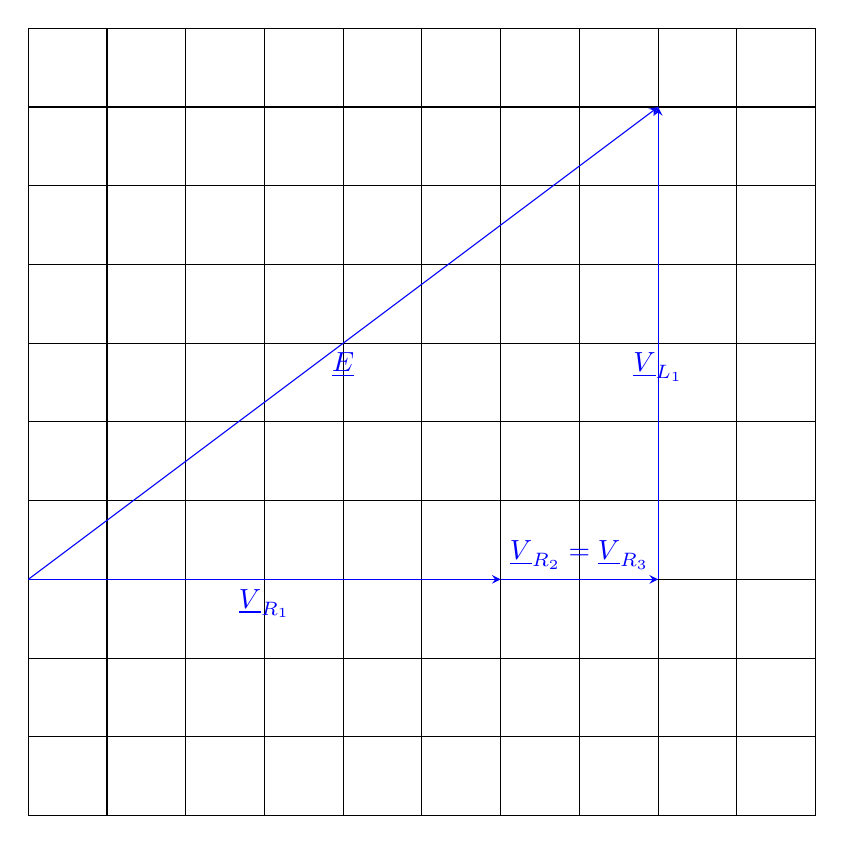
\begin{tikzpicture}
\draw (0,0) grid[step=1] (10,10);
\draw[-stealth, blue] (0,3)--(6,3) node[midway, below]{$\underline{V}_{R_1}$};
\draw[-stealth, blue] (6,3)--(8,3) node[midway, above]{$\underline{V}_{R_2}=\underline{V}_{R_3}$};
\draw[-stealth, blue] (8,3)--(8,9) node[midway, below]{$\underline{V}_{L_1}$};
\draw[-stealth, blue] (0,3)--(8,9) node[midway, below]{$\underline{E}$};
\end{tikzpicture}
\end{center}
}

\subsection{Question de l'Examen d'Août 2014}

\begin{center}
\begin{circuitikz} \draw
(0,0)   node [ground] {}
		to[sinusoidal voltage source, v=$V_i$] (0,3)
		to[R, l=$R$]						 (4,3)
		to[L, l=$L$]						 (4,0)
		to[R, l=$R_e$]						 (0,0)
(1,3) node[circ]{A}
(1,0) node[circ]{B}
(3,0) node[circ]{C}
;
\end{circuitikz}
\end{center}

Avec $R=2\Omega$, $R_e=1\Omega$, $L=5,5mH$ et $f=50Hz$.
\Question
{%Q
\textit{En utilisant la tension $\underline{V}_{CB}=1V*e^{j0^o}$ comme référence, donner l'expression des phaseurs $\underline{V}_{AB}$ et $\underline{V}_{AC}$.}
}
{%A
On trouve \underline{I} grâce à $\underline{V}_{CB}$ qui est donné: $$\underline{I}=\frac{\underline{V}_{CB}}{R_e}=1A*e^{j0^o}$$
Connaissant le courant et les impédances, par la loi d'Ohm:
$$\underline{V}_{AB}=(R+R_e+j\omega L)\underline{I}=(R+R_e+j\omega L)\frac{\underline{V}_{CB}}{R_e}=3+j2\pi 50*5,5*10^{-3}=3+j\sqrt{3}$$
$$\underline{V}_{AC}=(R+j\omega L)\frac{\underline{V}_{CB}}{R_e}=2+j2\pi 50*5,5*10^{-3}=2+j\sqrt{3}$$
}


\subsection{Question 7}
\begin{center}
\begin{circuitikz} \draw
(1,0)   to[R, l=$R_3$] 						(-1,2)
		to[R, l=$R_4$]    					(1,4)
		to[R, l=$R_1$]	            	    (3,2)
		to[R, l=$R_2$]	   					(1,0) -- (6,0)
(3,2) -- (6,2)
(1,4) -- (1,5)
		to[sinusoidal voltage source, v=$E$](5,5) -- (5,2)
node[circ] (B) at (6,0) {B}
node[circ] (A) at (6,2) {A}
(B) to [open, v_=$\underline{V}_{Th}?\ Z_{Th}?$] (A)
;
\end{circuitikz}
\end{center}

Soit le circuit représenté ci-dessus dont deux nœuds ont été nommés A et B pour la clarté de l’énoncé et dont les paramètres sont donnés ci-dessous:
\begin{itemize}
	\item $\underline{E}=6V.e^{j0°}$
	\item $R_1=5\Omega, R_2=4\Omega, R_3=6\Omega, R_4=10\Omega$
\end{itemize}
\vspace{5mm}
%QUESTION 1.1.
\Question
{
\textit{Calculer l'équivalent de Thévenin vu par l’accès AB.}
}
{%answer
La source $\underline{V}_{Th}$ se calcule en trouvant la tension à l'accès AB à vide.\\
Il suffit de calculer le diviseur d'impédance:
$$V_{AB}=V_{Th}=\frac{R_2}{R_2+R_3+R_4}V_i=\frac{6}{5}V$$

$$\fbox{V_{Th}=\frac{6}{5}V=1,2V$}$$

$Z_{Th}$ se calcule en court-circuitant la source. On a:
$$Z_{Th}=R_2//(R_3+R_4)=\frac{1}{\frac{1}{R_2}+\frac{A}{R_3+R_4}}=\frac{1}{\frac{1}{4}+\frac{1}{16}}=\frac{16}{5}$$
$$\fbox{Z_{Th}=\frac{16}{5}=3,2V}$$

}


%QUESTION 1.2.

\begin{center}
\begin{circuitikz} \draw
(1,0)   to[R, l=$R_3$] 						(-1,2)
		to[R, l=$R_4$]    					(1,4)
		to[R, l=$R_1$]	            	    (3,2)
		to[R, l=$R_2$]	   					(1,0)
(3,2) -- (6,2)
(1,4) -- (1,5)
		to[sinusoidal voltage source, v=$e(t)$, i_>=$i(t)$](4,5) 
		
(4.5,5) node[spdt] (Sw) { }
(Sw.in) node[ left ] {}
(Sw.out 1) node[right] {C} -- (6,5.3) -- (6,2)
(Sw.out 2) node[right] {D} to[L, l=$L_1$]       (5.1,2)
;
\end{circuitikz}
\end{center}

Soit le circuit ci-dessus repris de la question 1, pour lequel: $L_1=6,37mH=\frac{20}{\pi}mH$ et  $f=50Hz$.
\begin{itemize}
	\item Avant l'instant $t_1=0$, la source $e(t)=0V$ et l'interrupteur est connecté à la borne C.
	\item Au temps $t_1=0$, on active la source $e(t)=6V \sin(\omega t)$ et l'interrupteur reste connecté à C.
	\item Au temps $t_2=100ms$, l'interrupteur passe (de manière instantanée) de la borne C à la borne D.
\end{itemize}
\vspace{3mm}

\Question
{
\textit{Calculer le courant $i(t)$ délivré par la source $e(t)$ pour tout temps $t$.}
}
{%answer
\begin{enumerate}
\item de $t_1$ à $t_2$, il n'y a que des résistances, donc pas de transitoire. On calcule la résistance équivalente du montage:
$$R=R_1//(R_2+R_3+R_4)=4\Omega$$
Et donc,
$$i(t\in[t_1;t_2])=\frac{3}{2}\sin(\omega t)$$
\item en $t\geq t_2$. On devra connaitre les conditions de $i(t_2)$. Facile car $\sin(\omega t_2)=0$.
$$e(t)=Ri(t)+L\frac{di}{dt} \Rightarrow i(t) = Ae^{-\frac{R}{L}t}+i_P$$
$$\underline{I}_P=\frac{\underline{E}}{R+j\omega L}\Rightarrow i_P(t)=\frac{E}{\sqrt{R^2+(\omega L)^2}} \sin(\omega t - \theta)$$
avec $$\theta=arctan(\frac{\omega L}{R})$$
%\begin{itemize}
%	\item $Z=R4+2j\Omega$\\
%	$i_R(t)=\frac{6}{4+2j}\sin(\omega t)=(1,2-0,6)\sin(\omega t)$ pour $t\in[t_2;t_\infty]$
%	\item valeur en transitoire + régime\\
%	$i(t)=\frac{6}{\sqrt{4^2+2^2}}[\sin(\omega t)+26,6°+\sin(26,6°)\exp^{2t})]$
%\end{itemize}
Avec les conditions initiales, on obtient:
$$i(t) = \frac{E}{\sqrt{R^2+(\omega L)^2}}(sin(\omega t-\theta)-e^{-\frac{R}{L}t}sin(\theta))$$
\end{enumerate}

En conclusion:
$$i(t)=1,5A\sin(\omega t)\ pour\ t\in[0;100ms]$$
$$i(t)=2\sqrt{5}A[\sin(\omega t-26,6°)+\sin(26,6°)e^{-2t}])\ pour\ t\in[100ms;\infty]$$
}

\subsection{Question de l'Examen d'Août 2014}
\begin{center}
\begin{circuitikz} \draw
(0,0)   to[american voltage source, l=$e(t)$, i^>=$i(t)$, invert] 	(0,5)
		to[L, l=$L_1$]    				(3,5)
		to[L, l=$L_2$]	                (3,2.5)
		to[R, l=$R$]	   				(3,0) -- (0,0)
(3,5) -- (5,5)
to[american current source, l_=$i_S(t)$]  (5,0) -- (3,0)			
node (A) at (5.5,1) {}
node (B) at (5.5,4) {}
(A) to [open, v_=$v(t)$] (B)
%node[circ] (C) at (0.8,4.8) {}
%node[circ] (D) at (2.8,3) {}
%(D) to [open, v^=$M$] (C)
%(C) to [open, v=$ $] (D)
;
\end{circuitikz}
\end{center}

\vspace{-5mm}
Soit le circuit représenté ci-dessus comportant:\\
\begin{itemize}
	\item Une source de tension $e(t)=E_{0}+E_{1}\cos(\omega_1 t)$\\
	avec $E_0=3V$, $E_1=5V$ et $\omega_1=1000 rad/s$;
	\item Une source de courant $i_{s}(t)=I_{s}\sin(\omega_2 t+\phi)$\\
	avec $I_S=1A$, $\omega_2=2000 rad/s$ et $\phi=30°$;
	\item $R=1\Omega$, $L_1=2mH$, $L_2=1mH$.
\end{itemize}
\vspace{5mm}

On cherche à déterminer la tension $v(t)$ en régime établi.

%QUESTION 2.1.
\Question
{
%question
\textit{Quelles vont être les étapes de votre démarche afin de résoudre ce circuit et de trouver la tension $v(t)$ en régime établi?\\
Détaillez votre démarche sans recourir aux équations. }
}
{
\begin{itemize}
	\item \textbf{Définir les courants et tensions} sur le schéma \textbf{en respectant les conventions} générateur/récepteur
	\item Utiliser le \textbf{principe de superposition}: \textbf{pour chacun des 3 cas} ($\omega=0$, $\omega=\omega_1$ et $\omega=\omega_2$):
	\begin{itemize}
		\item \textbf{Simplification du schéma}\\
			Inductance = court-circuit en continu, source de tension nulle = court-circuit, source de courant nulle = circuit ouvert.
		\item \textbf{Exprimer les grandeurs en phaseurs} car nous cherchons la tension de régime
		\item \textbf{Equations de Kirchhoff}\\
			Loi des mailles: La somme algébrique des tensions aux bornes des branches constituant une maille est nulle.\\
			Loi des noeuds: La somme algébrique des courants quittant un noeud est nulle.
		\item \textbf{Résolution de l'équation/du système d'équations} par les méthodes algébriques classiques.
		\item Exprimer le résultat \textbf{dans le domaine temporel}.
	\end{itemize}
	\item Effectuer la \textbf{superposition}, c'est-à-dire sommer les 3 réponses temporelles.
\end{itemize}
}


%QUESTION 2.2.
\Question
{
\textit{Déterminer la tension $v(t)$ en régime établi.\\
\textbf{Pour vos calculs}: Ne pas déterminer les valeurs des arctangentes (laisser sous la forme $\arctan{x}$) et utiliser si besoin les approximations suivantes: $\sqrt{185} \approx 14$ et $\frac{4}{37} \approx 0,1$.}
}
{%answer
Puisque le circuit comporte 3 sources de pulsations différentes, l'utilisation du théorème de superposition est nécessaire.\\

\fbox{$\omega=0rad/s$}\\
En régime continu, les inductances se comportent comme des courts-circuits. En ne gardant que la source de tension $E_0$ et en annulant les deux autres sources, on obtient en phaseurs: $v_0=RI=E_0=3V$
\begin{center}
\begin{circuitikz} \draw
(0,0)   to[american voltage source, l=$e(t)$, i^>=$i(t)$, invert] 	(0,3)
		--    				(3,3)
		
		to[R, l=$R$]	   				(3,0) -- (0,0)
(3,3) -- (5,3)
to[open]  (5,0) -- (3,0)			
node (A) at (5.5,0) {}
node (B) at (5.5,3) {}
(A) to [open, v_=$v_0(t)$] (B)
%node[circ] (C) at (0.8,4.8) {}
%node[circ] (D) at (2.8,3) {}
%(D) to [open, v^=$M$] (C)
%(C) to [open, v=$ $] (D)
;
\end{circuitikz}
\end{center}

\fbox{$\omega=\omega_1=1000rad/s$}\\
En ne gardant que la source de tension $E_{1}\cos(\omega_1 t)$ et en annulant les deux autres sources, on obtient le circuit suivant:
\vspace{-5mm}
\begin{center}
\begin{circuitikz} \draw
(0,0)   to[american voltage source, l=$E_1 \cos(\omega_1 t)$, i^>=$i(t)$, invert] 	(0,5)
		to[L, l=$L_1$]    				(3,5)
		to[L, l=$L_2$]	                (3,2.5)
		to[R, l=$R$]	   				(3,0) -- (0,0)
(3,5) -- (5,5)
to[open]  (5,0) -- (3,0)			
node (A) at (5.5,1) {}
node (B) at (5.5,4) {}
(A) to [open, v_=$v_1(t)$] (B)
%node[circ] (C) at (0.8,4.8) {}
%node[circ] (D) at (2.8,3) {}
%(D) to [open, v^=$M$] (C)
%(C) to [open, v=$ $] (D)
;
\end{circuitikz}
\end{center}

Ce diviseur impédant donne l'expression suivante:\\
$\underline{V}_1=\frac{R+j\omega_1 L_2}{R+j\omega_1 (L_1+L_2)}\underline{E}_1$\\
$\underline{V}_1=\frac{1+j}{1+3j}\underline{E}_1=\frac{4-2j}{10}\underline{E}_1=\frac{2-j}{5}\underline{E}_1=\frac{\sqrt{5}}{5}\exp(-j \arctan \frac{1}{2}) E_1 \exp (j0°)=\sqrt{5}\exp(-j \arctan \frac{1}{2})$\\

%$\underline{E_1}=(R+j\omega_1 (L_1+L_2-2M))  \underline{I}$\\
%$\underline{V_1}=(R+j\omega_1(L_2-M)) \underline{I}$\\
%$\Leftrightarrow$\\
%$\underline{I}=\frac{\underline{E_1}}{R+j\omega_1 (L_1+L_2-2M)} $\\
%$\underline{V_1}=\frac{R+j\omega_1(L_2-M)}{R+j\omega_1 (L_1+L_2-2M)}\underline{E_1}=\frac{1+j}{1+2j}\underline{E_1}=\frac{3-j}{5}\underline{E_1}\\
%=\frac{\sqrt{10}}{5}\exp{(-j \arctan{\frac{1}{3}})}E_1\exp{(j0°)}=\frac{\sqrt{10}}{5}5\exp{(-j \arctan{\frac{1}{3}})}$\\

Et donc, dans le domaine temporel:\\
$v_1(t)=\sqrt{5}cos(1000t-\arctan{\frac{1}{2}})$

\fbox{$\omega=\omega_2=2000rad/s$}\\
En ne gardant que la source de courant $i_{s}(t)=I_{s}\sin(\omega_2 t+\phi)$ et en annulant les deux autres sources, on obtient le système de trois équations à trois inconnues suivant (2 équations de maille et 1 équation de noeud):\\
\shorthandoff{:!}
\begin{center}
\begin{circuitikz} \draw
(0,0)   to[short , i_=$i_1(t)$] 	(0,5)
		to[L, l=$L_1$, v<=$v_{L_1}$]    				(3,5)
		to[L, l=$L_2$, v>=$v_{L_2}$]	                (3,2.5)
		to[R, l=$R$, v>=$v_R$, i<_=$i_2(t)$]	   				(3,0) -- (0,0)
(3,5) -- (5,5)
to[american current source, l_=$i_S(t)$]  (5,0) -- (3,0)			
node (A) at (5.5,1) {}
node (B) at (5.5,4) {}
(B) to [open, v^<=$v_2(t)$] (A)
%node[circ] (C) at (0.8,4.8) {}
%node[circ] (D) at (2.8,3) {}
%(D) to [open, v^=$M$] (C)
%(C) to [open, v=$ $] (D)
;
\end{circuitikz}
\end{center}
\shorthandon{:!}
%\begin{center}
%	\includegraphics[width=8cm]{circuit_mutuelle_omega2.png}
%\end{center}


    $$\underline{V}_{L_1} = \underline{V}_{R}+\underline{V}_{L_2}$$
    $$\underline{V}_2 = -(\underline{V}_{R}+\underline{V}_{L_2})$$
    $$\underline{I_s} = \underline{I_1}+\underline{I_2}$$


Donc, $\underline{V}_2=-\underline{V}_{L_1}=-j \omega_2 L_1 \underline{I}_1$ et il nous suffit de trouver $\underline{I_1}$ en fonction de $\underline{I}_S$.\\

$$\underline{V}_{L_1} = \underline{V}_{R}+\underline{V}_{L_2}$$
$$\Rightarrow j \omega_2 L_1 \underline{I}_1=(R+j\omega_2 L_2) \underline{I}_2=(R+j\omega_2 L_2) (\underline{I}_S-\underline{I}_1)$$
$$\Rightarrow (R+j \omega_2 (L_1+L_2)) \underline{I}_1=(R+j\omega_2 L_2) \underline{I}_S$$
$$\Rightarrow \underline{I}_1=\frac{R+j\omega_2 L_2}{R+j \omega_2 (L_1+L_2)} \underline{I}_S$$
$$\Rightarrow \underline{V}_2=-\underline{V}_{L_1}=-j \omega_2 L_1 \underline{I}_1=-j \omega_2 L_1\frac{R+j\omega_2 L_2}{R+j \omega_2 (L_1+L_2)} \underline{I}_S$$

Numériquement:\\
$$\underline{V}_2=-4j \frac{1+2j}{1+6j}\underline{I}_S=4\frac{(2-j)}{1+6j}\underline{I}_S=4\frac{(2-j)(1-6j)}{1^2+6^2}\underline{I}_S=-4\frac{4+13j}{37}\underline{I}_S$$

Avec le phaseur $\underline{I_s}=I_s e^{j\phi}=1A e^{j30°}$, on obtient:
$$\underline{V_2}=-\frac{4}{37}\sqrt{4^2+13^2}e^{(j(30°+\arctan{\frac{13}{4}))}}=-\frac{4}{37}\sqrt{185}e^{(j(30°+\arctan{3,25})} \\ \approx -1,4 e^{(j(30°+\arctan{3,25})}$$

Et donc, dans le domaine temporel:
$$v_2(t)=-1,4 \sin(2000t+30°+\arctan{3,25})$$

Par le théorème de superposition, on a la solution finale $v(t)=v_0+v_1(t)+v_2(t)$:
$$\fbox{v(t)=3+\sqrt{5}cos(1000t-\arctan{\frac{1}{2}})-1,4 \sin(2000t+30°+\arctan{3,25})}$$
}


\end{document}